\documentclass[12pt]{article}
\title{Project 1}
\author{Eirik Ramsli Hauge\\
Joakim Kalsnes
}
\date{\today}

\usepackage{hyperref}
\usepackage{amsmath}
\usepackage[utf8]{inputenc}
\usepackage[english]{babel} 
%\usepackage{fullpage} 
\usepackage{amsfonts} 
\usepackage{amssymb} 
\usepackage{verbatim} 
 
\usepackage{color} 
\usepackage{setspace} 
\usepackage{blindtext}
\usepackage{epstopdf} 
\usepackage{braket}

\usepackage{cite} 
\usepackage{caption}
\usepackage{subcaption}
\usepackage{upgreek}
\usepackage{array,multirow}
\usepackage{pdfpages}

\usepackage{graphicx} 
\usepackage{float}

\usepackage{nameref}
\usepackage{hhline}
\usepackage{xtab}
\usepackage{booktabs, makecell, longtable}
\usepackage{lscape}

\newcommand{\E}[1]{\cdot 10^{#1}}
\newcommand{\e}[1]{\text{#1}}
\newcommand{\husk}[1]{\color{red} #1 \color{black}}


\DeclareMathOperator*{\argmin}{argmin}
\usepackage{bm}

\begin{document}
\maketitle

\begin{abstract}
Something smart
\end{abstract}
\section{Introduction}   \label{s:i}

\section{Theory}   \label{s:t}
The following section follows closely the notation and derivation of linear models and the bootstrap in Hastie et al. chapter 3.2, 3.4 and 7.11. \cite{Hastie2017}.
\subsection{Linear regression}
In this project we will use different linear methods for regression. Linear regression is a linear approach to modelling the relationship between a response variable (also known as dependent variable) and one or multiple predictor (independent) variables. Given the input vector (predictor variables) $X^T = (X_1, X_2,...., X_p)$, a linear regression model predicts the output via the model
\begin{equation} \label{eq:lin_reg}
f(X) = \beta_{0} + \sum_{j=1}^{p}X_j\beta_{j}
\end{equation}
The $\beta_j$'s are unknown coefficients, and are what we are trying to estimate. The variables $X_j$ can come from different sources. They can for instance be quantitative inputs, transformations of the inputs or polynomials of the inputs such as $X_3 = X_2^2$ and $X_4 = X_1^2X_2$. No matter the source of the $X_j$, the model is linear in the parameters.
\subsubsection{Least squares method}
Let us say we have a set of training data $(x_1,y_1),....,(x_N,y_N)$ from which we want to estimate the parameters $\beta$. Each $x_i = (x_{i1},x_{i2},...,x_{ip})^T$ is a vector of measurements for the $i$th case. The least squares method chooses the coefficients $\beta = (\beta_0,\beta_1,...,beta_p)^T$ by minimizing the residual sum of squares
\begin{equation} \label{eq:least_squares}
\begin{split}
RRS(\beta) &= \sum_{i=1}^{N}(y_i-f(x_i))^2\\
&= \sum_{i=1}^{N}(y_i-\beta_0-\sum_{j=1}^{p}x_{ij}\beta_j)^2.
\end{split}
\end{equation}
If we denote by $\bm{X}$ the $N\times(p+1)$ matrix with each row an input vector (with a 1 in the first position), and let $\bm{y}$ be the N-vector of outputs in the training set, we can write the residual sum of squares as
\begin{equation}
RRS(\beta) = (\bm{y}-\bm{X}\beta)^T(\bm{y}-\bm{X}\beta).
\end{equation}
Differentiating with respect to $\beta$ gives
\begin{equation}
\frac{\partial RSS}{\partial \beta} = -2\bm{X}^T(\bm{y}-\bm{X}\beta)
\end{equation}
\begin{equation}
\frac{\partial^2RSS}{\partial \beta \partial \beta^T} = 2\bm{X}^T\bm{X}.
\end{equation}
We set the first derivative to zero (assuming that $\bm{X}$ has full column rank)
\begin{equation}
\bm{X}^T(\bm{y}-\bm{X}\beta) = 0
\end{equation}
to obtain the unique solution
\begin{equation}
\hat{\beta} = (\bm{X}^T\bm{X})^{-1}\bm{X}^T\bm{y}.
\end{equation}
This gives the predicted value at an input vector $x_0$ as $\hat{f}(x_0)=(1:x_0)^T\hat{\beta}$, and the fitted values at the training inputs:
\begin{equation}
\hat{\bm{y}}=\bm{X}\hat{\beta}=\bm{X}(\bm{X}^T\bm{X})^{-1}\bm{X}^T\bm{y},
\end{equation}
where $\hat{y_i}=\hat{f}(x_i)$.\\ \\

\subsubsection{MSE, bias and variance}
One way of assessing the goodness of a model fit is by calculating the $mean\ squared\ error$ (MSE).
\begin{equation}
MSE = \frac{1}{N}\sum_{i=1}^{N}(y_i-\hat{f}(x_i))^2
\label{eq:MSE}
\end{equation}
This MSE can be decomposed into bias and variance.
\begin{equation}
\begin{split}
MSE &= E[(y-\hat{f}(x))^2] = Bias(\hat{f}(x))^2 + Var(\hat{f}(x)) + \sigma^2\\
&= (E[f(x)-\hat{f}(x)]^2) + (E[\hat{f}(x)^2]-E[\hat{f}(x)]^2) + \sigma^2
\end{split}
\end{equation}
The bias term measures how much the model, $\hat{f}(x)$, differs from the actual function, $f(x)$. A high bias means the model is underfitting the data. The model is not complex enough to capture all the information. On the other hand, a model can be overfitting. This happens when we use a very complex model that fits the training data very well. This model will have a high variance because it will be very sensitive to small fluctuations in the training set. As we can see, there is a trade-off between bias and variance. A simple model will have high bias and low variance, while a complex model will have low bias and high variance. The best model, i.e. lowest MSE, will be somewhere in the middle between a very simple and very complex model. In this project the bias and variance were calculated using the bootstrap technique (explained later).

\subsubsection{Shrinkage methods}
The least squares method is an intuitive and simple to understand-model, but the estimates obtained using this model are often not satisfactory. One of the reasons for this is the prediction accuracy. Least squares estimates often have low bias but large variance. By sacrificing a bit of bias to reduce the variance of the predicted values, the overall prediction accuracy may be improved. This can sometimes be done by setting some regression coefficients to zero or by shrinkage methods. Ridge regression and Lasso regression are examples of shrinkage methods.\\
Ridge regression shrinks the regression by imposing a penalty proportional to the square of the magnitude of the coefficients. To find the ridge coefficients, the penalized residual sum of squares is minimized.
\begin{equation}
\hat{\beta}^{ridge}=\argmin_{\beta}\{\sum_{i=1}^{N}(y_i-\beta_0-\sum_{j=1}^{p}x_{ij}\beta_j)^2+\lambda\sum_{j=1}^{p}\beta_j^2\}
\label{eq:ridge}
\end{equation}
The $\lambda\geq0$ parameter controls the amount of shrinkage, with increasing amount of shrinkage as $\lambda$ increases. A problem using the least squares method is that when there are many correlated predictor variables, their coefficients may become poorly determined and exhibit high variance. "A wildly large positive coefficient on one variable can be canceled by a similarly large negative coefficient on its correlated cousin." (Hastie p. 63). By imposing a penalty as in Ridge regression, this problem is reduced.\\
When performing a ridge regression it is common to use centered inputs. That is, each $x_{ij}$ is replaced by $x_{ij} - \bar{x}_j$. $\beta_0$ is estimated by $\bar{y}=\frac{1}{N}\sum_{1}^{N}y_i$, and the remaining coefficients get estimated by a ridge regression using centered inputs. We can write equation \ref{eq:ridge} in matrix form:\\
\begin{equation}
RSS(\lambda) = (\bm{y}-\bm{X}\beta)^T(\bm{y}-\bm{X}\beta)+\lambda\beta^T\beta.
\end{equation}
This gives the ridge regression solutions:
\begin{equation}
\hat{\beta}^{ridge} = (\bm{X}^T\bm{X}+\lambda\bm{I})^{-1}\bm{X}^T\bm{y},
\end{equation}
where $\bm{I}$ is the $p\times{p}$ identity matrix. By adding a positive constant to the diagonal of $\bm{X}^T\bm{X}$ before inversion the problem is made nonsingular, even if $\bm{X}^T\bm{X}$ is not of full rank.\\ \\
Another shrinkage method is the lasso. The lasso method is quite similar to ridge regression, but with some differences. We can write the lasso regression problem as
\begin{equation}
\hat{\beta}^{lasso}=\argmin_{\beta}\{\frac{1}{2}\sum_{i=1}^{N}(y_i-\beta_0-\sum_{j=1}^{p}x_{ij}\beta_j)^2+\lambda\sum_{j=1}^{p}\left|\beta_j\right|\}.
\label{eq:lasso}
\end{equation}
Equivalently, it can be written as
\begin{equation}
\begin{split}
\hat{\beta}^{lasso}=&\argmin_{\beta}\sum_{i=1}^{N}(y_i-\beta_0-\sum_{j=1}^{p}x_{ij}\beta_j)^2\\
&subject\ to\ \sum_{j=1}^{p}\left|\beta_j\right|\leq{t}.
\end{split}
\end{equation}
If $t$ is sufficiently small the nature of the constraint will cause some of the coefficients to be exactly zero. Thus, the lasso does a kind of continuous subset selection. The penalty parameter in both lasso and ridge regression should be chosen to minimize an estimate of the expected prediction error.\\
\subsection{Bootstrapping}
The bootstrap is a general tool used in statistics for assigning measures of accuracy to sample estimates. These measures of accuracy can for instance be defined in terms of bias, variance, prediction error or confidence intervals. Bootstrapping can be applied to a lot of statistical problems, e.g. hypothesis testing, model comparison and model optimization.\\
Say we have a model fit to a set of training data denoted by $\bm{Z}=(z_1,z_2,...,z_N)$ where $z_i = (x_i,y_i)$. The basic idea of the bootstrap is then to randomly draw datasets with replacement from the training set, where each sample has the same size as the original training set. This is done B times, producing B bootstrap datasets. For each bootstrap dataset we refit the model, and examine the behaviour of the quantities of interest. For instance the mean squared error, the r$^2$ score and the values of the $\beta$s can be computed for each dataset. This gives distributions of the quantities, and these distributions can be assessed by for instance mean and confidence intervals.
\section{Experimental}   \label{s:e}
All scripts used in this project can be found on github at \url{https://github.com/eirikraha/fysstk3155---Project-1}. By running the script named \texttt{taska.py} one must use one or two additional command line arguments. Each of these arguments will be described in turn below, but a brief summary is given in table \ref{tabE:sum}:
\begin{table}[H]
\centering
\begin{tabular}{c|p{12cm}}
\textbf{Arguments} & \textbf{Function} \\ \hline
a & Runs an ordinary least square regression analysis on the data produced by the Frankie Function. The data is also analyzed using bootstrap. \\ \hline
b & Runs a Ridge regression analysis on the data produced by the Frankie Function. The data is also analyzed using bootstrap. \\ \hline
b plot & Same as above, but one also produces a plot to visually determine the optimal $\lambda$. \\ \hline
c & Runs a Lasso regression analysis on the data produced by the Frankie Function. The data is also analyzed using bootstrap. \\ \hline
c plot & Same as above, but one also produces a plot to visually determine the optimal $\alpha$. \\ \hline
d & Imports map data from the file \texttt{SRTM\_data\_Norway\_1.tif} and plots the terrain data as a colormap in gray scale. \\ \hline
e & Imports map data from the file \texttt{SRTM\_data\_Norway\_1.tif} and divides the data into patches before performing ordinary least squared, ridge and lasso regression using bootstrap to find the optimal regression analysis.
\end{tabular}
\caption{Summary of the different command line arguments accepted. One can also use the argument "all" to do every command line in succession.}
\label{tabE:sum}
\end{table}
The command line arguments a, b and c all represents different regression analysis as described in section \ref{s:t}. However, the script requires data to work upon. These data are produced by the Frankie Function where we give in two vectors, $\bm{x}$ and $\bm{y}$ and produce an array of z-values. The vectors  $\bm{x}$ and $\bm{y}$ are defined to be in the interval $\bm{x}, \bm{y} \in [0,1]$ and are uniformally distributed. Furthermore, one also needs the matrix $\bm{X}$ which contains all the functions we will allow the regression analysis to use in combination to recreate the data. For this project we will usually use combinations of $\bm{x}$ and $\bm{y}$ up to polynomials of fifth order.
\subsection{Command Line Argument: a}
Given the command line argument "a" the script will use the data from the Frankie Function and $\bm{X}$ to perform an ordinary least square regression analysis. This analysis is done on noise free and noisy data both by a home made function created using the linear algebra presented in section \ref{s:t} and using the LinearRegression function from \texttt{scikit learns}. The condifidence interval of $\beta$ is also found. Afterwards, R2 and MSE is calculated by the function \texttt{R2MSEeval} where one can choose to use either \texttt{scikit learns} or home made functions. Lastly, the script performs bootstrapping upon data with and without noise, evaluating for R2, MSE, bias and variance.
\subsection{Command Line Argument: b and c with or without plot}
The command line arguments "b" and "c" will do the same as "a" only using Ridge and Lasso regression respectively. If one adds the command line argument "plot" the script will produce plots of the R2 and MSE for different values of $\lambda$ and $\alpha$. These plots are then again used to finde the optimal and stable value for $\lambda$ and $\alpha$. For Lasso, one has to use the function provided from \texttt{scikit learn} as there is no home made function to be used.
\subsection{Command Line Argument: d}
This command line argument provides a part of the script which is more used as a proof of concept. By providing "d" as your argument, the class \texttt{terrainReader} will import the map data stored in the file \texttt{SRTM\_data\_Norway\_1.tif} and plot it. This is a general method which can be used for all \texttt{.tif}-files downloaded from \url{https://earthexplorer.usgs.gov/}.
\subsection{Command Line Argument: e}
Lastly, the commmand line argument "e" will provide you with a combination of all the tasked performed previously. The script will now read the map data, divide it into a set number of patches and perform ordinary least square, ridge and lasso regression using bootstrap. The MSE, R2, bias and variance will then be calculated for each method.


\husk{Adding noise og kanskje Franke Function i teori?}
\section{Results and Discussion}  \label{s:rd}
All results which are either written to file or plotted can be found in the \texttt{benchmarks} and \texttt{figures} folders. \\ \\
Using command line argument "a", "b" and "c" we performed different methods for regression upon our data and found the results presented in table \ref{tabR:abc}.
\begin{table}[H]
\centering
\begin{tabular}{c|c|c|c|c|c|c|c}
Method & R2 & MSE & $\lambda$ & $\alpha$ & Variance & Bias & Error \\ \hline
OLS & $0.976$ & $1.94\E{-3}$ & - & - & - & - & - \\ \hline
Ridge & $0.977$ & $2.08\E{-3}$ & $1\E{-4}$ & - & - & - & - \\ \hline
Lasso &  $0.659$ & $3.16\E{-2}$ & - & $1\E{-2}$ & - & - & - \\ \hline
OLS* & $0.976$ & $1.94\E{-3}$ & - & - & - & - & - \\ \hline
Ridge* & $0.977$ & $2.07\E{-3}$ & $1\E{-4}$ & - & - & - & - \\ \hline
Lasso* &$0.659$ & $3.16\E{-2}$ & - & $1\E{-2}$ & - & - & -  \\ \hline
OLS$^{\dagger}$ & $0.975$ & $1.97\E{-3}$ & - & - & $1.01\E{-5}$ & $1.96\E{-3}$ & $1.97\E{-3}$ \\ \hline
Ridge$^{\dagger}$ & $0.977$ & $2.07\E{-3}$ & $1\E{-4}$ & - & $8.26\E{-6}$ & $2.06\E{-3}$ & $2.07\E{-3}$ \\ \hline
Lasso$^{\dagger}$ & $0.664$ & $3.05\E{-2}$ & - & $1\E{-2}$ & $1.79\E{-5}$ & $3.05\E{-2}$ & $3.05\E{-2}$  \\ \hline
\end{tabular}
\caption{Results from OLS, Ridge and Lasso regression on data from the Franke Function, data from the Franke Function with added noise of 0.01 (*) and by using bootstrap with 1000 iterations ($\dagger$). - symbolises values not relevant or nonexisting.}
\label{tabR:abc}
\end{table}
As we can see there are small differences between ordinary least squared and Ridge, however Lasso seems to be the biggest looser. It is evident that the noise contribution is too small to make any difference and should be increased for a more in depth study of its effect. By bootstrapping we can see that the R2-score and MSE are relatively stable. The bias and variance have big differences for all three methods with Bias being the main contributor to the error. \husk{Er ikke dette litt rart i og med at Lasso og Ridge skal bytte på å ha high/low variance og low/high bias?}. \\ \\
Given the subpar MSE and R2-score of the Lasso-method it would be natural to change the $\alpha$ value until we receive satisfactory results. This can also be done to the $\lambda$ in the Ridge method and figure \ref{figRD:RLR2MSE} illustrates the R2-score and the MSE for different values:
\begin{figure}[H]
\centering
\begin{subfigure}[t]{0.48\textwidth}
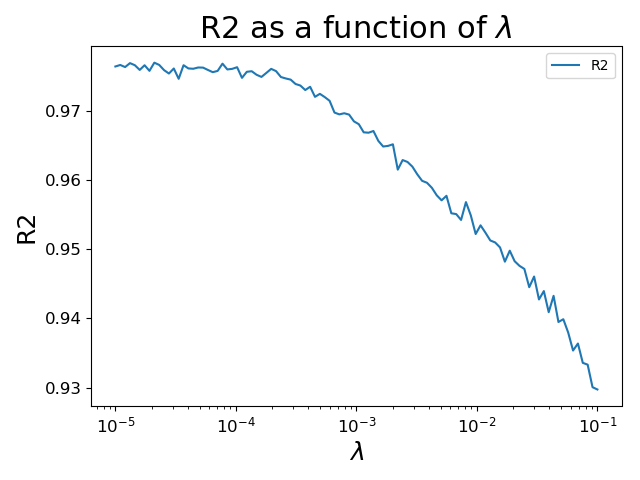
\includegraphics[width=\linewidth]{../figures/RidgeR2.png}
\caption{Ridge R2}
\label{figRD:RR2}
\end{subfigure}
\ \
\begin{subfigure}[t]{0.48\textwidth}
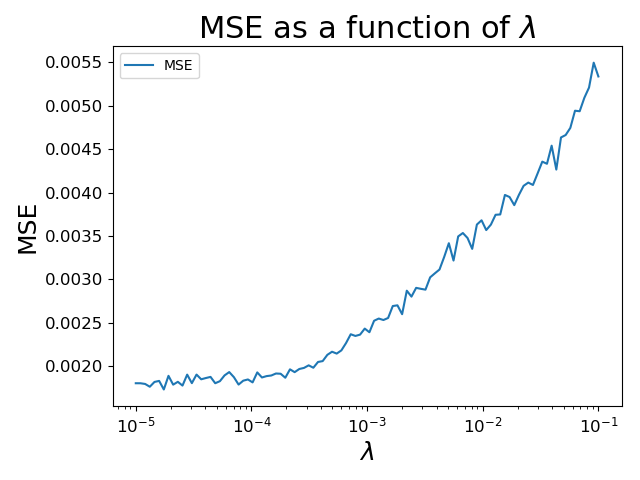
\includegraphics[width = \linewidth]{../figures/RidgeMSE.png}
\caption{Ridge MSE}
\label{figRD:RMSE}
\end{subfigure}
\\
\begin{subfigure}[t]{0.48\textwidth}
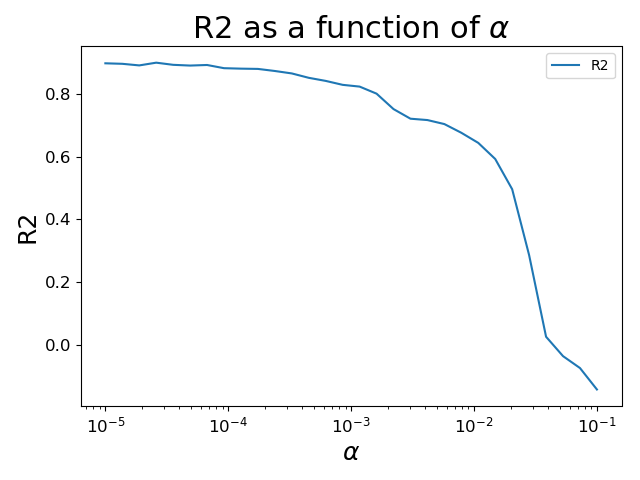
\includegraphics[width=\linewidth]{../figures/LassoR2.png}
\caption{Lasso R2}
\label{figRD:LR2}
\end{subfigure}
\
\begin{subfigure}[t]{0.48\textwidth}
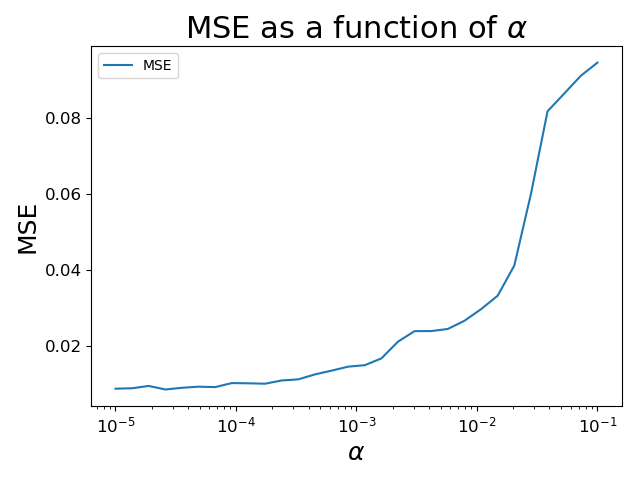
\includegraphics[width = \linewidth]{../figures/LassoMSE.png}
\caption{Lasso MSE}
\label{figRD:LMSE}
\end{subfigure}
\caption{R2-scores and MSE for different values of $\lambda$ and $\alpha$ using Ridge and Lasso respectively.}
\label{figRD:RLR2MSE}
\end{figure}
From these values we found that the optimal $\lambda$ was a bit above $1\E{-4}$ as this is before the start of a major fall for R2 and a major rise for MSE. Going below this value seems to have little to no effect upon both R2 and MSE. Similarily with $\alpha$ we can see that $\E{-2}$ right below a major climb/fall in MSE and R2 respectively. There also seems to be something to be gained going below this value, however doing this gives a warning from \texttt{scikit learn} saying that going too low may cause precision problems. $\alpha = 1\E{-2}$ is therefore a compromise between good enough scores and precision. One could argue the use of a lower $\alpha$, however, to ensure reproducible results, this high $\alpha$ was chosen. These are also the values used for the calculations in table \ref{tabR:abc}.

\husk{Colorplot med støy og alpha/lambda på aksene? Hadde vært kult.}

\husk{Analyse av hvilken metode som er best}


\section{Future Works}\label{s:fw}
\section{Conclusion}  \label{s:con}
\section*{References} \label{s:ref}
\section*{Appendix A} \label{app:A}
\end{document}